\Needspace{0.30\textheight}
\section{Vue 2: cú pháp và cơ chế hoạt động}

\textbf{Component} là một đơn vị giao diện có dữ liệu, hành vi và phần hiển thị riêng.
\textbf{State} là dữ liệu hiện tại của component. \textbf{Props} là dữ liệu đầu vào
do component cha truyền xuống component con; thông báo đi ngược lên qua
\textbf{event}, tức sự kiện do
component phát ra. \textbf{Reactivity (cơ chế phản ứng)} là khả năng Vue theo dõi
sự thay đổi của state và tự động cập nhật phần giao diện phụ thuộc vào state đó.

\figref{fig:vue-props-events} thể hiện luồng giao tiếp giữa hai component: component
cha truyền dữ liệu xuống bằng props; component con phát event để component cha nhận
thông báo và quyết định cách cập nhật state.

\begin{center}
\resizebox{0.52\textwidth}{!}{\begin{tikzpicture}[
  every node/.style={font=\small,align=center},
  part/.style={draw,rounded corners=1.5mm,minimum width=42mm,minimum height=9mm,thick},
  group/.style={draw=blue!60,rounded corners=2mm,thick,inner sep=4mm},
  arrow/.style={-{Latex[length=2mm]},very thick}
]
\node[font=\small\bfseries,text=blue!60!black] (ptitle) {Component cha};
\node[part,fill=blue!12,draw=blue!55,below=3mm of ptitle] (pstate) {State\\dữ liệu do component cha quản lý};
\node[part,fill=green!12,draw=green!55!black,below=3mm of pstate] (pmethods) {Methods\\xử lý hành vi và cập nhật state};
\node[part,fill=orange!12,draw=orange!70!black,below=3mm of pmethods] (ptemplate) {Template / UI\\hiển thị dữ liệu};
\node[group,fit=(ptitle)(pstate)(pmethods)(ptemplate)] (parentbox) {};

\node[font=\small\bfseries,text=blue!60!black,right=65mm of ptitle] (ctitle) {Component con};
\node[part,fill=blue!12,draw=blue!55,below=3mm of ctitle] (cstate) {State\\dữ liệu riêng của component con};
\node[part,fill=green!12,draw=green!55!black,below=3mm of cstate] (cmethods) {Methods\\xử lý tương tác người dùng};
\node[part,fill=orange!12,draw=orange!70!black,below=3mm of cmethods] (ctemplate) {Template / UI\\hiển thị và nhận tương tác};
\node[group,fit=(ctitle)(cstate)(cmethods)(ctemplate)] (childbox) {};

\draw[arrow,draw=blue!65] (pstate.east) --
  node[midway,above=1.5mm,text=blue!65!black,font=\small\bfseries] {props}
  (cstate.west);
\node[font=\scriptsize,text=blue!55!black] at
  ($(pstate.east)!0.5!(cstate.west)+(0,-4mm)$) {cha truyền dữ liệu xuống con};

\draw[arrow,draw=orange!80!black] (cmethods.west) --
  node[midway,above=1.5mm,text=orange!80!black,font=\small\bfseries] {event}
  (pmethods.east);
\node[font=\scriptsize,text=orange!70!black] at
  ($(cmethods.west)!0.5!(pmethods.east)+(0,-4mm)$) {con dùng \texttt{\$emit} để báo cho cha};

\node[below=6mm of $(ptemplate.south)!0.5!(ctemplate.south)$,font=\small]
  {Mỗi component quản lý giao diện riêng; component cha là nguồn dữ liệu chính của props};
\end{tikzpicture}
}
\captionof{figure}{Luồng props và event giữa component cha và component con}
\label{fig:vue-props-events}
\end{center}

\subsection{Cấu trúc Single-File Component và Options API}

Các component có thể ghép với nhau. Vue thường lưu mỗi component trong một
\textbf{Single-File Component} (file \texttt{.vue}) gồm:

\begin{itemize}
  \item \texttt{<template>} mô tả cấu trúc giao diện bằng HTML và directive của Vue;
  \item \texttt{<script>} xuất ra đối tượng cấu hình component;
  \item \texttt{<style>} chứa CSS và có thể dùng thuộc tính \texttt{scoped} để giới
  hạn style trong component.
\end{itemize}

\textbf{Options API} tổ chức đối tượng cấu hình theo loại trách nhiệm:

\begin{itemize}
  \item \texttt{props} khai báo dữ liệu component cha được phép truyền xuống;
  \item \texttt{data} trả về state riêng của mỗi đối tượng component được tạo;
  \item \texttt{computed} khai báo giá trị được suy ra từ state hoặc props;
  \item \texttt{methods} chứa hành vi được gọi trực tiếp, thường từ sự kiện;
  \item \texttt{watch} theo dõi một giá trị để chạy tác vụ phụ khi giá trị đổi.
\end{itemize}

\subsection{Các cú pháp chính}

\textbf{DOM} là cây các phần tử HTML do trình duyệt quản lý. \textbf{Directive} là
thuộc tính đặc biệt bắt đầu bằng \texttt{v-}, yêu cầu Vue áp dụng một hành vi lên
DOM. Các dạng viết tắt \texttt{:} và \texttt{@} lần lượt thay
cho \texttt{v-bind:} và \texttt{v-on:}.

{\small
\begin{longtable}{|>{\raggedright\arraybackslash}p{0.21\textwidth}|
                  >{\raggedright\arraybackslash}p{0.33\textwidth}|
                  >{\raggedright\arraybackslash}p{0.36\textwidth}|}
\caption{Các cú pháp Vue 2 thường dùng}\label{tab:vue-syntax}\\
\hline
\textbf{Cú pháp} & \textbf{Nó làm gì?} & \textbf{Khi nào dùng?} \\
\hline
\texttt{\{\{ value \}\}} & Chuyển giá trị thành text an toàn trong template. & Hiển thị tên, trạng thái hoặc số liệu. \\
\hline
\texttt{v-if}/\texttt{v-else} & Tạo hoặc hủy nhánh DOM theo điều kiện. & Nội dung ít chuyển trạng thái hoặc không nên tồn tại khi điều kiện sai. \\
\hline
\texttt{v-for} + \texttt{:key} & Tạo một nhánh giao diện cho mỗi phần tử; key giúp Vue nhận diện từng phần tử qua các lần dựng giao diện. & Danh sách, lựa chọn hoặc hàng trong bảng. \\
\hline
\texttt{v-bind}/\texttt{:} & Gán biểu thức JavaScript vào attribute hoặc prop. & Truyền \texttt{:items}, \texttt{:disabled} hoặc dữ liệu cho component con. \\
\hline
\texttt{v-on}/\texttt{@} & Đăng ký hàm xử lý sự kiện. & \texttt{@click}, \texttt{@input} hoặc \texttt{@submit.prevent}. \\
\hline
\texttt{v-model} & Kết hợp truyền giá trị và lắng nghe sự kiện cập nhật theo quy ước. & Ô nhập, danh sách chọn hoặc component biểu mẫu tự viết. \\
\hline
\end{longtable}
}

Trong Vue 2, \texttt{v-model} trên custom component mặc định kết hợp prop
\texttt{value} với sự kiện \texttt{input}. Component nhận giá trị từ cha và phát
\texttt{this.\$emit('input', newValue)} khi cần cập nhật
\cite{vue2-template,vue2-components}.

\subsection{Ví dụ component}

Component \texttt{PatientPicker} nhận danh sách bệnh nhân qua prop, lọc theo từ khóa
bằng \texttt{computed} và phát sự kiện \texttt{select} khi người dùng chọn một bệnh
nhân. Các directive và dạng viết tắt trong ví dụ đã được trình bày ở mục trước.

\lstinputlisting[basicstyle=\ttfamily\fontsize{7.4}{8.1}\selectfont]
  {../../examples/vue2/PatientPicker.vue}

Ví dụ thể hiện quy ước \textbf{props down, events up}: component cha truyền dữ liệu
xuống bằng prop \texttt{patients}; component con không sửa prop mà phát event bằng
\texttt{\$emit} để cha quyết định hành động tiếp theo. Cách này giữ một nguồn chịu
trách nhiệm thay đổi dữ liệu và làm luồng dữ liệu dễ theo dõi
\cite{vue2-components}.

Ví dụ được build thành bản production bằng Vite. \figref{fig:vue2-code-output}
ghi lại kết quả chạy thật sau khi nhập ``Thảo'' và chọn bệnh nhân được lọc.

\begin{center}
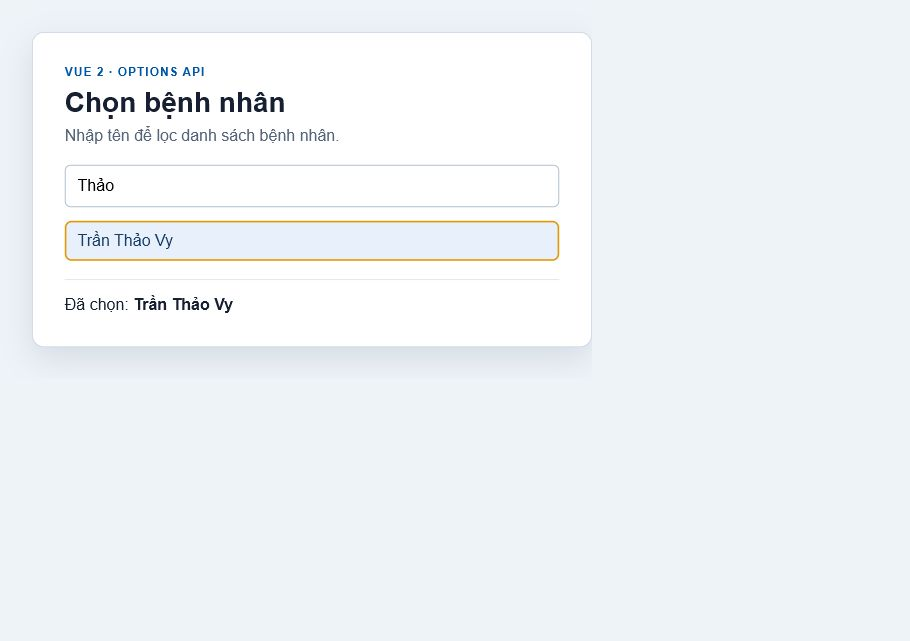
\includegraphics[width=0.64\textwidth,trim=0 270 280 0,clip]
  {../../assets/code-output/vue2-patient-picker-output.png}
\captionof{figure}{Kết quả chạy component \texttt{PatientPicker} sau khi build}
\label{fig:vue2-code-output}
\end{center}

\Needspace{0.24\textheight}
\subsection{Phân biệt methods, computed và watch}

\textbf{Tác vụ phụ} (side effect) là hành động không chỉ trả về một giá trị, chẳng
hạn gọi API, ghi bộ nhớ trình duyệt hoặc sửa state khác.

{\small
\begin{longtable}{|>{\raggedright\arraybackslash}p{0.18\textwidth}|
                  >{\raggedright\arraybackslash}p{0.34\textwidth}|
                  >{\raggedright\arraybackslash}p{0.38\textwidth}|}
\caption{Phân biệt methods, computed và watch}\label{tab:vue-options}\\
\hline
\textbf{Option} & \textbf{Bản chất} & \textbf{Ví dụ phù hợp} \\
\hline
\texttt{methods} & Hàm chạy mỗi lần được gọi; có thể thay đổi state hoặc phát sự kiện. & Xử lý click, gửi biểu mẫu hoặc gọi một hành động rõ ràng. \\
\hline
\texttt{computed} & Giá trị suy ra được lưu lại; chỉ tính lại khi state hoặc prop đã đọc bên trong thay đổi. & Danh sách đã lọc, tổng tiền hoặc trạng thái nút dựa trên nhiều trường dữ liệu. \\
\hline
\texttt{watch} & Theo dõi một giá trị và chạy tác vụ phụ khi giá trị đó đổi. & Gọi API tìm kiếm sau khi người dùng ngừng nhập trong một khoảng ngắn, ghi log hoặc đồng bộ với hệ thống bên ngoài. \\
\hline
\end{longtable}
}

Vì computed nên chỉ mô tả giá trị suy ra, tác vụ phụ thuộc về method hoặc watch. Nếu
có thể biểu diễn một giá trị bằng
computed thì không cần dùng watch để chép dữ liệu từ chỗ này sang chỗ khác
\cite{vue2-computed}.

\subsection{Cơ chế reactivity và cập nhật DOM}

Khi một đối tượng Vue 2 được tạo, Vue duyệt các thuộc tính đã khai báo trong
\texttt{data} và chuyển mỗi thuộc tính thành getter/setter bằng
\texttt{Object.defineProperty}:

\begin{itemize}
  \item \textbf{getter} chạy khi code đọc thuộc tính;
  \item \textbf{setter} chạy khi code gán giá trị mới cho thuộc tính;
  \item \textbf{dependency} là thuộc tính mà giao diện đã đọc và phụ thuộc vào;
  \item \textbf{watcher} là đối tượng theo dõi các dependency của component và được
  thông báo khi một dependency thay đổi.
\end{itemize}

Luồng cập nhật giao diện diễn ra theo thứ tự trong \figref{fig:vue-render-flow}:

\begin{center}
\resizebox{0.90\textwidth}{!}{\begin{tikzpicture}[
  node distance=3.2mm,
  every node/.style={font=\scriptsize,align=center},
  flowbox/.style={draw,rounded corners=1.5mm,minimum height=25mm,minimum width=20.5mm,text width=18mm,thick},
  number/.style={circle,fill=orange!80!black,text=white,font=\scriptsize\bfseries,inner sep=1.4mm},
  arrow/.style={-{Latex[length=1.8mm]},thick,draw=orange!80!black}
]
\node[flowbox,fill=orange!12,draw=orange!70!black] (s1) {State\\thay đổi};
\node[flowbox,fill=orange!8,draw=orange!70!black,right=of s1] (s2) {Getter/setter\\của Vue 2\\phát hiện};
\node[flowbox,fill=green!12,draw=green!55!black,right=of s2] (s3) {Watcher\\được\\thông báo};
\node[flowbox,fill=blue!10,draw=blue!55,right=of s3] (s4) {Render\\function\\chạy lại};
\node[flowbox,fill=violet!10,draw=violet!60,right=of s4] (s5) {Tạo\\Virtual DOM\\mới};
\node[flowbox,fill=blue!8,draw=blue!55,right=of s5] (s6) {So sánh diff\\và tạo\\bản vá patch};
\node[flowbox,fill=green!12,draw=green!55!black,right=of s6] (s7) {DOM thật / UI\\được cập nhật};

\foreach \a/\b in {s1/s2,s2/s3,s3/s4,s4/s5,s5/s6,s6/s7}
  \draw[arrow] (\a) -- (\b);

\node[number,above=2mm of s1] (n1) {1};
\node[number,above=2mm of s2] (n2) {2};
\node[number,above=2mm of s3] (n3) {3};
\node[number,above=2mm of s4] (n4) {4};
\node[number,above=2mm of s5] (n5) {5};
\node[number,above=2mm of s6] (n6) {6};
\node[number,above=2mm of s7] (n7) {7};

\node[draw=orange!70!black,dashed,rounded corners=1.5mm,below=7mm of s2,text width=43mm,minimum height=12mm]
  (detectnote) {Vue 2 dùng getter/setter để biết dependency nào đã thay đổi};
\draw[dashed,-{Latex[length=1.6mm]},draw=orange!70!black]
  (s2.south) -- (detectnote.north);

\node[draw=green!55!black,rounded corners=1.5mm,fill=green!8,below=7mm of s6,text width=50mm,minimum height=12mm,font=\small\bfseries,text=green!45!black]
  (resultnote) {Chỉ phần giao diện chịu ảnh hưởng được cập nhật};
\draw[dashed,-{Latex[length=1.6mm]},draw=green!55!black]
  (s7.south) -- (resultnote.north east);
\end{tikzpicture}
}
\captionof{figure}{Luồng Vue 2 ghi nhận thay đổi và cập nhật DOM}
\label{fig:vue-render-flow}
\end{center}

Template được biên dịch thành \textbf{hàm dựng giao diện} (render function). Khi watcher chạy lại, hàm
này tạo một cây \textbf{Virtual DOM}, tức biểu diễn JavaScript nhẹ của giao diện.
Vue thực hiện \textbf{diff} để so sánh cây mới với cây trước, sau đó \textbf{patch}
những thay đổi cần thiết vào DOM thật. Cách này tránh xây lại toàn bộ trang mỗi khi
một giá trị đổi.

Vue không cập nhật DOM ngay sau từng phép gán. Các watcher được đưa vào một hàng đợi;
nếu cùng watcher bị kích hoạt nhiều lần trong một lượt xử lý JavaScript, Vue chỉ giữ
một lần. Lượt xử lý kế tiếp gọi là \textbf{tick}; khi đó Vue xử lý hàng đợi và cập
nhật DOM. Khi code cần đọc
DOM sau cập nhật, dùng \texttt{await this.\$nextTick()}
\cite{vue2-instance,vue2-reactivity}.

\subsection{Giới hạn reactivity với object và array}

Vue 2 tạo getter/setter cho các thuộc tính tồn tại lúc đối tượng khởi tạo. Nếu thêm
một thuộc tính mới bằng phép gán thông thường, Vue không có setter cho thuộc tính đó
nên không biết phải thông báo watcher. \texttt{\$set} vừa thêm thuộc tính vừa đăng ký nó
vào hệ thống reactivity:

\Needspace{0.14\textheight}
\begin{lstlisting}
// Sai neu "note" chua ton tai luc khoi tao:
this.patient.note = 'VIP'

// Dung:
this.$set(this.patient, 'note', 'VIP')
\end{lstlisting}

Tương tự, Vue 2 không phát hiện chắc chắn phép gán trực tiếp theo index của array.
Dùng \texttt{\$set} hoặc một phương thức biến đổi mảng mà Vue đã bọc, chẳng hạn
\texttt{splice}:

\Needspace{0.10\textheight}
\begin{lstlisting}
this.$set(this.rows, index, updatedRow)
// hoac:
this.rows.splice(index, 1, updatedRow)
\end{lstlisting}

Cách đơn giản nhất vẫn là khai báo trước cấu trúc chính của state trong \texttt{data};
\texttt{\$set} dùng cho trường hợp thực sự cần thêm thuộc tính động
\cite{vue2-reactivity}.
